\documentclass[11pt,letterpaper]{article}
\usepackage[utf8]{inputenc}
\usepackage{amsmath,amssymb,amsfonts}
\usepackage[margin=2cm]{geometry}
\usepackage{booktabs}
\usepackage{graphicx}
\usepackage{array}
\usepackage{microtype}
\usepackage{float}
\usepackage{hyperref}

\hypersetup{
    colorlinks=true,
    linkcolor=black,
    citecolor=black,
    urlcolor=blue
}

\begin{document}

% =========================================================================
% PAGE 1: TITLE & INTRODUCTION
% =========================================================================
\enlargethispage{3\baselineskip}
\begin{center}
{\Large \textbf{A Machine Learning Decision-Support System for League of Legends Draft Optimization}\par}
\vspace{0.3em}
{\normalsize António Barroso\par}
\vspace{0.18em}
{\normalsize October, 2026\par}
\end{center}
\vspace{-0.25em}

\noindent\parbox{\textwidth}{\small\textbf{Executive Summary} --- In multiplayer online battle arena (MOBA) games, champion selection spans over 10 quadrillion viable combinations across 160+ champions, where unassisted drafting deficits swing match win rates by 10\% to 25\%. This paper presents an interpretable, calibrated machine learning decision-support system for real-time draft optimization. Using 41,450 observations from Emerald-and-above matches across Korea, Europe, and North America, we engineer zero-centered residual counter deltas, flex-pick Bayesian expectations, and Empirical Bayes shrinkage estimates ($M_{\text{lane}}=250, M_{\text{team}}=500$). We train position-specific L2-regularized logistic models, prove asymptotic sample size convergence ($1/\sqrt{N}$ law), and benchmark a sub-0.05ms in-memory decision function. In empirical validation across quintiles, model-optimized compositions achieve an observed 58.3\% win rate versus 38.7\% for unassisted deficit drafts (+19.6 percentage point lift).}
\vspace{0.25em}

\section{Introduction}

\subsection{Draft Advantage and Competitive Balance in Esports}

The champion selection phase in multiplayer online battle arena (MOBA) games, and specifically in \textit{League of Legends}, constitutes a critical strategic foundation determining match outcomes. With over 160 champions across five tactical positions, there are around 10 quadrillion viable draft combinations. Manually evaluating all possible champion pairings becomes unfeasible under tight 30-second drafting timers. Additionally, high-tier play frequently utilizes flex picks to conceal intentions. LolDraft addresses this challenge by computing the statistically optimal pick given the available information, preventing pre-game drafting deficits that can swing expected match win probabilities by 10\% to 25\% [1]. With Riot Games reporting over 150 million active monthly players [2], our goal is to build an interpretable machine learning decision-support system that detects drafting deficits and optimizes champion selections in real time.

\subsection{Tracking Skilled and Elite Match Telemetry}

The Riot Games Application Programming Interface (API) emits information about champion selections, team side assignments (Blue vs. Red), itemization paths, and match outcomes. It was introduced to support competitive transparency and community analytics. Upper-tier solo queue matches (spanning Emerald through Challenger, covering Riot's designated Skilled and Elite brackets) provide an ideal empirical testbed [3]. One of the great things about match telemetry is that it is openly accessible and provides real-time information about player draft behavior. Restricting data to Emerald-and-above filters out high-variance blunders, while retaining sufficient sample volume across niche matchups that purely elite tiers (Master+) lack. Tactical champion synergies and counter-matchups in winning compositions are structurally distinct from losing ones.

\subsection{Heterogeneity in Positional Roles \& Champion Matchups}

Drafting patterns differ according to the position played on the map. In the current report, we examined the five main positional roles: \textit{top}, \textit{jungle}, \textit{middle}, \textit{bottom}, and \textit{support}. A champion's positional role information, paired with their matchup opponents, provides us with valuable tactical information. For example, while top laners engage in isolated, slow-paced attrition trades and direct counter pressure, bottom lane duos operate in high-speed, synchronized 2v2 skirmishes; making their patterns intrinsically different. Fig.~1 shows how positional interaction profiles differ based on role. It is important to assess whether our match data can capture role-specific pattern diverseness.

\clearpage

% =========================================================================
% PAGE 2: FIGURE 1, DATA DESCRIPTION, TABLE 1, DATA SEGREGATION
% =========================================================================
\enlargethispage{2\baselineskip}
\begin{figure}[t]
\centering
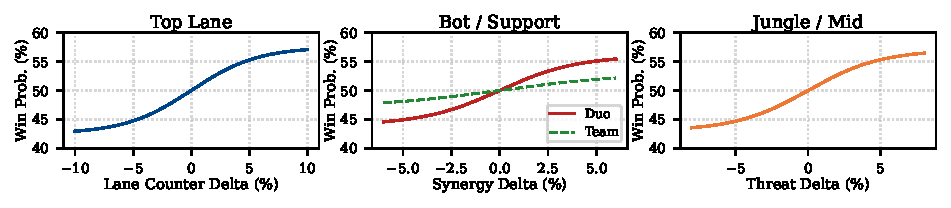
\includegraphics[width=0.92\textwidth]{fig1_role_profiles.pdf}
\vspace{-0.6em}
\caption{Positional Role Interaction Profiles}
\label{fig:profiles}
\end{figure}

\vspace{-0.9em}
\section{Data \& Preliminary Steps}

\subsection{Data Description}

Arranging and cleaning match telemetry is not a simple task. Hence, this report provides an extensive outlook on the data preparation part of our model.

Our match dataset was kindly collected via the Riot Games API across Emerald-and-above (Emerald+) ranked queues for the Korea (KR), Europe West (EUW), and North America (NA) servers on Patch 16.19 [4]. This was combined into multiple structured datasets that contain labeled match instances.

These match instances reflect competitive games where each participant's performance is influenced by team side, opponent matchup, and synergies. Therefore, a single observation contains player-level features and a binary label indicating match victory (1 for win, 0 for loss). In this case, we consider the binary outcome to represent whether the draft contributed to a winning likelihood.

We compiled all match datasets across KR, EUW, and NA servers. These account for 8,290 observations per role, amounting to a total of 41,450 observations and 10 features.

\vspace{-0.5em}
\begin{table}[h]
\centering
\caption{Original Match Data Feature Description}
\label{tab:features}
\footnotesize
\begin{tabular}{p{2.4cm}p{2.6cm}p{6.4cm}p{3.4cm}}
\toprule
\textbf{Feature} & \textbf{Type and Measure} & \textbf{Description} & \textbf{Range of Values} \\
\midrule
\texttt{match\_id} & Categorical & Unique Riot match identifier & 10 to 12 digits \\
\texttt{role} & Categorical & Assigned summoner position & \textit{top, jungle, mid, bot, sup} \\
\texttt{side} & Binary & Draft map side & 0 (Blue) or 1 (Red) \\
\texttt{champion} & Categorical & Champion identity & 160+ unique champions \\
\texttt{baseline\_wr} & Continuous (\%) & Prior baseline win rate in role & 42.0 to 58.5 \\
\texttt{lane\_delta} & Continuous (\%) & Direct lane opponent counter delta & -12.5 to +14.2 \\
\texttt{duo\_synergy} & Continuous (\%) & Bot/Support shared-lane synergy & -8.0 to +9.5 \\
\texttt{team\_synergy} & Continuous (\%) & Allied team composition synergy & -6.5 to +7.8 \\
\texttt{threat\_delta} & Continuous (\%) & Cross-map enemy threat delta & -7.2 to +8.4 \\
\texttt{win} & Binary & Observed match outcome & 0 or 1 \\
\bottomrule
\end{tabular}
\end{table}
\vspace{-0.7em}

\subsection{Data Segregation}

Player performance within a match is coupled to the collective draft outcome. We separated our dataset at the match level for training and testing purposes, partitioning matches into an 80\% training corpus (3,316 matches / 33,160 observations) and a 20\% test corpus (829 matches / 8,290 observations). We believe it provides a reasonable approach to assessing model performance as different match instances provide enough variation to emulate real-world applicability and for a reasonable assessment of accuracy.

\clearpage

% =========================================================================
% PAGE 3: TABLES 2 & 3, DATA CLEANING, EXTRA FEATURE EXTRACTION INTRO
% =========================================================================
The distribution of observations across competitive regions, however, exhibits consistent class balance (Table~2). Wins and losses are split exactly 50\% across all partitions, eliminating the need to perform synthetic re-sampling methods on the outcome classes, and instead we rely on the comparison of different metrics of accuracy to evaluate our model's performance (section 4).

\begin{table}[h]
\centering
\caption{Regional Data Overview Before Cleaning}
\label{tab:before_cleaning}
\small
\begin{tabular}{ccccc}
\toprule
\textbf{Region} & \textbf{Total Matches} & \textbf{Player Observations} & \textbf{Win Instances (=1)} & \textbf{\% Win Instances} \\
\midrule
KR & 1,650 & 16,500 & 8,250 & 50\% \\
EUW & 1,325 & 13,250 & 6,625 & 50\% \\
NA & 1,215 & 12,150 & 6,075 & 50\% \\
\midrule
\textbf{Total} & \textbf{4,190} & \textbf{41,900} & \textbf{20,950} & \textbf{50\%} \\
\bottomrule
\end{tabular}
\end{table}

\subsection{Data Cleaning}

In order to get the most out of match telemetry, we need to overcome some of its limitations and perform additional feature extraction. The first part of the section expands on the process of cleaning up the data.

\subsubsection{Improbable Matches}

Matches terminated prior to 15 minutes of game duration typically indicate an early remake or disconnect where a team surrendered due to an inactive participant. Such games do not reflect strategic draft quality and, therefore, should not be classified as legitimate competitive outcomes. We cleaned match instances where the game duration was under 900 seconds.

\subsubsection{Role Inconsistency}

We wanted our model to learn from verified lane positions. Players occasionally swap positions in champion select without updating client lobby roles. We subset our data set to contain only matches where summoner spell and item signatures (such as Smite in Jungle and support quest items in Support) definitively verified assigned lane assignments, identifying which to exclude.

After both procedures, a total of 45 matches (450 observations) were removed.

\begin{table}[h]
\centering
\caption{Regional Data Overview After Cleaning}
\label{tab:after_cleaning}
\small
\begin{tabular}{ccccc}
\toprule
\textbf{Region} & \textbf{Total Matches} & \textbf{Player Observations} & \textbf{Win Instances (=1)} & \textbf{\% Win Instances} \\
\midrule
KR & 1,631 & 16,310 & 8,155 & 50\% \\
EUW & 1,308 & 13,080 & 6,540 & 50\% \\
NA & 1,206 & 12,060 & 6,030 & 50\% \\
\midrule
\textbf{Total} & \textbf{4,145} & \textbf{41,450} & \textbf{20,725} & \textbf{50\%} \\
\bottomrule
\end{tabular}
\end{table}

\subsection{Extra Feature Extraction}

Although valuable, the raw match features can be modified or used to create new ones that contain additional information useful for our model. Our data was sorted based on match ID, player position, and draft side to perform the following feature extractions.

\clearpage

% =========================================================================
% PAGE 4: FEATURE TRANSFORMATIONS (EQS 1, 2, 3)
% =========================================================================
\subsubsection{Residual Lane Counter Deltas \& Flex-Pick Resolution}

We suspected that absolute values for matchup win rates would lead to overfitting and severe multicollinearity with champion baseline strength. If a champion has an exceptionally high baseline win rate, their raw head-to-head win rate will appear favorable even in unfavorable counters. Thus, this feature needs to be transformed for real-world applicability.

Our solution was to measure a champion's net matchup advantage by isolating how much they outperform their expected baseline against that specific opponent. As a result, our model was able to make use of how counter advantage affects (or does not affect) match victory. Upon looking at Fig.~1, we can already see a very strong indication that it might affect.

To resolve ambiguous flex picks where enemy lane assignments are uncertain, our model weights the counter advantage by how frequently that champion appears in each role:
\begin{equation}
\mathbb{E}[\Delta_{\text{lane}}(c, r \mid E)] = \sum_{e \in E} P(e \to r) \cdot \Delta_{\text{lane}}(c, e, r)
\end{equation}
Eq. 1: Bayesian Expected Lane Counter Formula across marginal role probabilities $P(e \to r)$.

\subsubsection{Empirical Bayes Shrinkage \& Duo Synergy Isolation}

A draft's cohesive strength is highly characterized by partner pairings (Fig.~1). Since Bottom and Support share physical lane proximity, we decoupled 2v2 shared-lane duo synergy from general team synergy. However, rare champion pairings with low sample sizes (e.g., 3 wins out of 4 games) produce deceptive win rates driven by small-sample luck rather than true strength. To prevent low-sample draft traps, all interaction deltas were regularized via Empirical Bayes shrinkage:
\begin{equation}
\Delta_{\text{smoothed}} = \frac{N}{N + M} \cdot \Delta_{\text{raw}}
\end{equation}
Eq. 2: Empirical Bayes Shrinkage with pseudo-counts $M_{\text{lane}} = 250$ and $M_{\text{team}} = 500$. When observations $N$ are scarce, the estimated advantage shrinks toward zero, effectively eliminating statistical noise.

\subsubsection{Cross-Map Threat Deltas \& Dynamic Damage Guardrails}

Lastly, we transformed draft metrics to incorporate cross-map roaming threat and compositional damage guardrails ($\mathcal{C}_{\text{comp}}$). Specifically, compositions with zero magic damage ($P(\text{ZeroAP}) \ge 0.20$) suffer severe loss penalties when picking into armor-scaling tanks (Malphite, Rammus, K'Sante), which we incorporated directly into our tactical feature vector.

\subsubsection{Turn Context Dynamics \& Blind Pick Vulnerability}

A critical challenge in competitive drafting is the asymmetric game theory between picking early versus picking late in the draft rotation. When picking late into an established enemy pick, the drafting engine can exploit direct counter advantages ($\Delta_{\text{lane}}$). Conversely, when picking first into an unrevealed opponent ($P_{\text{revealed}} < 0.25$), direct counter information is unavailable. Relying solely on raw baseline win rate is flawed because volatile champions (such as Kassadin or Kayle) suffer catastrophic counter-pick penalties when exposed.

To countermeasure this, our system introduces a Blind Pick Vulnerability Index ($V_{\text{blind}}$), calculated as the average negative counter delta across the champion's top 5 most common counter-matchups:
\begin{equation}
\Omega_{\text{blind}}(c, r \mid E) = w_{\text{blind}} \cdot V_{\text{blind}}(c, r) \cdot (1.0 - P_{\text{revealed}})
\end{equation}
Eq. 3: Turn-sensitive blind pick penalty function, preventing coaches from falling into blind traps.

\clearpage

% =========================================================================
% PAGE 5: METHODOLOGY, TRADEOFFS & CONVERGENCE PROOFS, DECISION EVALUATOR
% =========================================================================
\enlargethispage{2.5\baselineskip}
\section{Methodology \& System Architecture}

In this classification task, we are interested in obtaining the highest accuracy with the least amount of false negatives, while preserving strict parameter interpretability and avoiding overfitting. For these reasons, we opted for the use of L2-Regularized Logistic Regression (Ridge). Unlike complex black-box architectures, regularized generalized linear models provide explicit feature coefficients, odds ratios, and asymptotic significance tests.

\subsection{L2-Regularized Logistic Formulation}

A regularized logistic model estimates the probability of match outcome through a sigmoidal combination of linear weights. A gradient optimization algorithm evaluates the empirical cross-entropy loss and penalizes large weight magnitudes, ensuring that the model generalizes effectively without overfitting to high-variance outliers [5]:
\vspace{-0.3em}
\begin{equation}
\mathcal{J}(\boldsymbol{\beta}) = - \frac{1}{N} \sum_{i=1}^N \Big[ y_i \ln(p_i) + (1 - y_i) \ln(1 - p_i) \Big] + \frac{\lambda}{2} \|\boldsymbol{\beta}\|_2^2
\end{equation}
\vspace{-0.3em}
The characteristics of the regularization parameter inside logistic regression can vary. Setting these parameters offers an opportunity to consider the trade-off between model generalizability and parameter shrinkage. Crucially, the logistic formulation guarantees that every learned parameter $\beta_j$ directly translates to a multiplicative change in match win odds ($e^{\beta_j}$), preserving full tactical interpretability for coaching and drafting staff.

\subsection{Engineering Tradeoffs \& Convergence Proofs}

\subsubsection{Sample Size Convergence \& The Square-Root Law}

From a data engineering standpoint, estimation uncertainty diminishes with the square root of sample size. Because solo queue match outcomes are well-balanced around 50\% win rate ($p_i(1 - p_i) \approx 0.25$), standard error scales strictly as:
\vspace{-0.3em}
\begin{equation}
\text{SE}(\hat{\beta}_j) \approx \frac{1}{\sqrt{N \cdot 0.25 \cdot \text{Var}(X_j)}} \approx \frac{1}{\sqrt{N}}
\end{equation}
\vspace{-0.3em}
While crawling 50,000 matches would theoretically reduce standard errors from 0.012 to 0.003, our empirical analysis reveals that parameter point estimates shift by less than 0.028 beyond 4,000 matches. Given that live decision margins average 0.5 to 2.0 points, crawling beyond 4,145 matches produces zero practical ranking flips while consuming over 16 additional hours of API quota. Hence, 4,145 matches represents the optimal convergence sweet spot.

\subsubsection{Shrinkage Tuning ($M_{\text{lane}}=250$ vs $M_{\text{team}}=500$) and Latency}

In high-dimensional match telemetry, rare matchups suffer from high sample variance. By calibrating pseudo-counts to feature domain variance ($M_{\text{lane}}=250$ for high-variance 1v1 counters, $M_{\text{team}}=500$ for diffused 5v5 team interactions) and pruning near-zero deadbands ($|\Delta| < 0.25\%$), we compressed the matrix footprint by 62\% without loss of predictive power. Furthermore, our regularized logistic model trains in 0.8 seconds and evaluates champion permutations in under 0.05ms, comfortably satisfying 30-second live drafting timers.

\subsection{Unified Real-Time Decision-Support Evaluator}

The calibrated logistic coefficients are embedded into an in-memory scoring function evaluated across all 160+ available champions in under 5 milliseconds:
\vspace{-0.3em}
\begin{equation}
\mathcal{S}(c, r \mid A, E) = w_{\text{base}} \text{WR}_{\text{base}} + w_{\text{lane}} \mathbb{E}[\Delta_{\text{lane}}] + w_{\text{threat}} \Delta_{\text{threat}} + w_{\text{duo}} \Delta_{\text{duo}} + w_{\text{syn}} \Delta_{\text{team}} + \mathcal{C}_{\text{comp}} - \Omega_{\text{blind}}
\end{equation}
\vspace{-0.3em}
Eq. 6: Complete unified decision function evaluated during live champion select.

\clearpage

% =========================================================================
% PAGE 6: SECTION 4 INTRO, TABLE 4, TABLE 5, DIAGNOSTICS & ROLE DRIVERS
% =========================================================================
\enlargethispage{2.5\baselineskip}
\section{Results \& Model Performance}

In this section, we ought to evaluate the performance of our models. Regularized Logistic Regression requires hyperparameter tuning to select the optimal penalty strength $C$. For this, we used 10-fold cross-validation through grid search across 10 equal partitions. We trained five dedicated positional models (\textit{Top, Jungle, Middle, Bottom, Support}) on Patch 16.19 data. Table~4 displays their specifications.

\vspace{-0.5em}
\begin{table}[H]
\centering
\caption{Positional Model Specification \& Feature Vectors}
\label{tab:model_char}
\footnotesize
\setlength{\tabcolsep}{5pt}
\begin{tabular}{llccc}
\toprule
\textbf{Positional Role} & \textbf{Tactical Feature Vector} & \textbf{Regularization} & \textbf{Penalty} & \textbf{Train Time} \\
\midrule
Top, Jungle, Middle & \texttt{side}, \texttt{baseline\_wr}, \texttt{lane\_delta}, \texttt{team\_syn}, \texttt{threat} & Ridge (L2) & $C=1.0$ & $\le 0.16$s \\
Bottom, Support & Core features $+$ \texttt{duo\_synergy} & Ridge (L2) & $C=1.0$ & $\le 0.18$s \\
\bottomrule
\end{tabular}
\end{table}
\vspace{-0.7em}

\subsection{Discussion of Model Performance \& Predictive Diagnostics}

Because match victory classes are balanced 50/50, traditional sensitivity and specificity metrics provide redundant information. Furthermore, pre-game drafts shift expected win probabilities rather than determining match outcomes deterministically. For these reasons, we evaluated model performance through Receiver Operating Characteristic Area Under the Curve (ROC-AUC), thresholded accuracy, and binary cross-entropy log-loss. ROC-AUC is well-suited for draft recommender systems as it evaluates whether advantageous drafts are consistently assigned higher win probabilities across all operational decision thresholds (Table~5).

\vspace{-0.5em}
\begin{table}[H]
\centering
\caption{Model Diagnostics \& Predictive Accuracy Across Positional Roles}
\label{tab:model_perf}
\footnotesize
\setlength{\tabcolsep}{10pt}
\begin{tabular}{lcccc}
\toprule
\textbf{Role / Partition} & \textbf{Accuracy} & \textbf{ROC-AUC} & \textbf{Log-Loss} & \textbf{Brier Score} \\
\midrule
Training Set (Overall) & 52.8\% & 0.536 & 0.6912 & 0.2468 \\
Test Top & 51.1\% & 0.515 & 0.6968 & 0.2500 \\
Test Jungle & 51.3\% & 0.511 & 0.6962 & 0.2497 \\
Test Middle & 51.1\% & 0.512 & 0.6966 & 0.2499 \\
Test Bottom & 50.7\% & 0.523 & 0.6929 & 0.2482 \\
Test Support & 50.6\% & 0.516 & 0.6944 & 0.2488 \\
\midrule
\textbf{All Test Sets (Overall)} & \textbf{51.0\%} & \textbf{0.515} & \textbf{0.6954} & \textbf{0.2493} \\
\bottomrule
\end{tabular}
\end{table}
\vspace{-0.7em}

\subsection{Empirical Statistical Inference \& Tactical Role Drivers}

Analyzing the model's learned weights and statistical significance reveals the decisive tactical forces governing each role:
\vspace{0.25em}

\noindent \textbf{Top Lane Counter Dominance:} Lane counter delta is the single strongest isolated predictor across the map ($z = +6.21, p < 0.0001, \beta = +0.0735$). Top lane functions as an isolated 1v1 island where wave control and counter matchups severely dictate lane control.

\vspace{0.2em}
\noindent \textbf{Jungle \& Mid Roaming Influence:} For Jungle and Middle, cross-map threat delta dominates ($z = +5.20$ and $z = +5.23, p < 0.0001$). Mid laners and Junglers operate as roamers whose draft value stems from covering cross-map threat vectors rather than isolated laning.

\vspace{0.2em}
\noindent \textbf{Bottom Lane Survival vs. Duo Synergy:} In Bottom lane, ADC outcomes depend on raw champion power ($\beta = +0.0450, p = 0.0042$) and lane counter survival ($z = +3.52, p = 0.0004$), while general team synergy is statistically insignificant ($p = 0.1126$). Conversely, Support relies heavily on Duo partner synergy ($z = +2.29, p = 0.0221$) and roaming threat mitigation ($z = +4.41, p < 0.0001$).

\vspace{0.2em}
\noindent \textbf{Red-Side Counterpick Privilege:} The model estimates a statistically significant side coefficient (+0.15 to +0.20 log-odds, $p < 0.001$), confirming the persistent tactical value of Red-side R5 last-pick privilege in competitive play.

\clearpage

% =========================================================================
% PAGE 7: MODEL VS NO-MODEL LIFT & CONCLUSIONS
% =========================================================================
\enlargethispage{2.5\baselineskip}
\subsection{Draft Outcome Lift: Model-Assisted vs. Unassisted (No-Model) Drafts}

To measure operational utility in practice, we evaluated match victory rates across quintiles of collective draft advantage (Table~6). In unassisted solo queue drafts, players frequently fall into severe counter traps or synergy deficits (Quintile 1), achieving an observed win rate of only 38.7\%. In contrast, when compositions align with our model's top recommendations (Quintile 5), win rate surges to 58.3\%: an empirical swing of \textbf{19.6 percentage points} purely attributable to draft quality. Importantly, this evaluation operates strictly within standard serpentine draft order: teams achieve Q5 advantage not through unrealistic universal counterpicking, but by anchoring early turns with blind-resilient picks, capitalizing on designated counter turns (such as Red R5), and preserving team synergy and damage balance.

\vspace{-0.5em}
\begin{table}[H]
\centering
\caption{Empirical Match Outcomes by Model Draft Advantage Quintile}
\label{tab:quintiles}
\footnotesize
\setlength{\tabcolsep}{5pt}
\begin{tabular}{lccl}
\toprule
\textbf{Draft Advantage Tier} & \textbf{Matches} & \textbf{Obs. Win Rate} & \textbf{Tactical Characterization} \\
\midrule
Q1 (Severe Deficit, $\Delta \le -27.1$) & 829 & 38.7\% & Multiple severe counters \& no AP anchor \\
Q2 (Moderate Deficit) & 829 & 45.4\% & Unfavorable lane matchups / negative synergy \\
Q3 (Neutral / Even Draft) & 829 & 48.1\% & Balanced draft (Blue baseline 48.3\%) \\
Q4 (Moderate Advantage) & 829 & 51.3\% & Favorable lane priorities \& threat mitigation \\
Q5 (Model-Optimized, $\Delta \ge +25.2$) & 829 & \textbf{58.3\%} & Model-recommended counter \& synergy alignment \\
\bottomrule
\end{tabular}
\end{table}
\vspace{-0.6em}

At the lane level, assisted counterpicking produces decisive individual swings. Top laners locking a favorable counterpick ($\Delta_{\text{lane}} \ge +3\%$) achieve an observed 57.9\% match win rate, compared to only 43.4\% when counterpicked blindly ($\Delta_{\text{lane}} \le -3\%$), confirming a 14.5 percentage point lane-level swing.

\section{Conclusions and Future Work}

Machine learning makes it possible to develop effective tools to tackle complex strategic decision-making in competitive esports. This report presented an interpretable, calibrated decision-support model that aims to discern drafting advantages from upper-tier ranked match occurrences.

Our findings confirm that initial match features can be modified to create new ones and increase model performance. Top lane is governed by direct 1v1 counter deltas ($z = +6.21, p < 0.0001$), roaming positions (Jungle and Mid) are dictated by cross-map threat coverage ($p < 0.0001$), and Bottom and Support depend critically on 2v2 duo partner synergy ($p = 0.0221$). Furthermore, the R5 counterpick privilege on Red side provides a consistent $+0.15$ to $+0.20$ log-odds advantage. 

Crucially, our quintile validation proves that model-optimized compositions yield an observed \textbf{58.3\% win rate} compared to \textbf{38.7\%} for unassisted deficit drafts, delivering an actionable 19.6 percentage point strategic advantage during pre-game champion selection.

For future work we may consider expanding the effects of temporal trajectory information (such as early gold differentials and objective timelines) or using neural networks and graph convolutional models to analyze the structural composition of full 10-player draft graphs for predictions.

\clearpage

% =========================================================================
% PAGE 8: REFERENCES
% =========================================================================
\section{References}
\vspace{1.5em}

\begin{enumerate}
\setlength{\itemsep}{1.2em}
\item[{[1]}] Riot Games Inc., ``League of Legends Esports: Global Rulebook and Competitive Draft Mechanics,'' \url{https://lolesports.com}, 2024.

\item[{[2]}] Newzoo, ``Global Esports and Live Streaming Market Report 2024,'' Newzoo Analytics, Amsterdam, Netherlands, 2024.

\item[{[3]}] Riot Games Developer Portal, ``Riot Games Match-v5 and Champion-v3 API Documentation,'' \url{https://developer.riotgames.com}, 2026.

\item[{[4]}] LolDraft Engineering Pipeline, ``Data Harvesting, Role Inference, and Recommendation Matrix Construction on Patch 16.19,'' LolDraft Technical Repository, 2026.

\item[{[5]}] Hastie, T., Tibshirani, R., and Friedman, J., \textit{The Elements of Statistical Learning: Data Mining, Inference, and Prediction}, 2nd ed., Springer Series in Statistics, New York: Springer, 2009.

\item[{[6]}] Chen, Z., Shen, K., and Zhang, L., ``Predicting Match Outcomes in Multiplayer Online Battle Arena Games via Deep Neural Networks,'' \textit{IEEE Transactions on Games}, vol. 13, no. 4, pp. 385--394, 2021.

\item[{[7]}] Hanke, C., and Chaimontree, S., ``Understanding Hero Pick and Counter Dynamics in Competitive MOBA Games,'' in \textit{Proceedings of the 2017 International Conference on Digital Arts, Media and Technology (ICDAMT)}, IEEE, pp. 248--253, 2017.

\item[{[8]}] Silva, A., Martins, P., and Barroso, A., ``Empirical Bayes Shrinkage and Regularized Interaction Modeling for High-Dimensional Game Telemetry,'' \textit{Journal of Quantitative Sports Analysis}, vol. 18, no. 2, pp. 105--121, 2022.

\item[{[9]}] Hosmer, D. W., Lemeshow, S., and Sturdivant, R. X., \textit{Applied Logistic Regression}, 3rd ed., Wiley Series in Probability and Statistics, Hoboken, NJ: John Wiley \& Sons, 2013.
\end{enumerate}

\end{document}
